% $Header: /u/gcmpack/manual/s_phys_pkgs/text/exch2.tex,v 1.21 2004/10/12 17:27:17 edhill Exp $
% $Name:  $

%%  * Introduction
%%    o what it does, citations (refs go into mitgcm_manual.bib, 
%%      preferably in alphabetic order)
%%    o Equations 
%%  * Key subroutines and parameters
%%  * Reference material (auto generated from Protex and structured comments)
%%    o automatically inserted at \section{Reference} 


\section{exch2: Extended Cubed Sphere \mbox{Topology}}
\label{sec:exch2}


\subsection{Introduction}

The \texttt{exch2} package extends the original cubed sphere topology
configuration to allow more flexible domain decomposition and
parallelization.  Cube faces (also called subdomains) may be divided
into any number of tiles that divide evenly into the grid point
dimensions of the subdomain.  Furthermore, the tiles can run on
separate processors individually or in groups, which provides for
manual compile-time load balancing across a relatively arbitrary
number of processors. \\

The exchange parameters are declared in
\filelink{pkg/exch2/W2\_EXCH2\_TOPOLOGY.h}{pkg-exch2-W2_EXCH2_TOPOLOGY.h}
and assigned in
\filelink{pkg/exch2/w2\_e2setup.F}{pkg-exch2-w2_e2setup.F}. The
validity of the cube topology depends on the \file{SIZE.h} file as
detailed below.  The default files provided in the release configure a
cubed sphere topology of six tiles, one per subdomain, each with
32$\times$32 grid points, with all tiles running on a single processor.  Both
files are generated by Matlab scripts in
\file{utils/exch2/matlab-topology-generator}; see Section
\ref{sec:topogen} \sectiontitle{Generating Topology Files for exch2}
for details on creating alternate topologies.  Pregenerated examples
of these files with alternate topologies are provided under
\file{utils/exch2/code-mods} along with the appropriate \file{SIZE.h}
file for single-processor execution.

\subsection{Invoking exch2}

To use exch2 with the cubed sphere, the following conditions must be
met:

\begin{itemize}
\item The exch2 package is included when \file{genmake2} is run.  The
  easiest way to do this is to add the line \code{exch2} to the
  \file{profile.conf} file -- see Section \ref{sect:buildingCode}
  \sectiontitle{Building the code} for general details.
  
\item An example of \file{W2\_EXCH2\_TOPOLOGY.h} and
  \file{w2\_e2setup.F} must reside in a directory containing files
  symbolically linked by the \file{genmake2} script.  The safest place
  to put these is the directory indicated in the \code{-mods=DIR}
  command line modifier (typically \file{../code}), or the build
  directory.  The default versions of these files reside in
  \file{pkg/exch2} and are linked automatically if no other versions
  exist elsewhere in the build path, but they should be left untouched
  to avoid breaking configurations other than the one you intend to
  modify.
  
\item Files containing grid parameters, named \file{tile00$n$.mitgrid}
  where $n$=\code{(1:6)} (one per subdomain), must be in the working
  directory when the MITgcm executable is run.  These files are
  provided in the example experiments for cubed sphere configurations
  with 32$\times$32 cube sides -- please contact
  \begin{rawhtml}
    <A href="mailto:mitgcm-support@dev.mitgcm.org"> 
  \end{rawhtml} 
\begin{verbatim}
MITgcm-support@mitgcm.org
\end{verbatim}
  \begin{rawhtml} </A> \end{rawhtml}
  if you want to generate files for other configurations.
  
\item As always when compiling MITgcm, the file \file{SIZE.h} must be
  placed where \file{genmake2} will find it.  In particular for exch2,
  the domain decomposition specified in \file{SIZE.h} must correspond
  with the particular configuration's topology specified in
  \file{W2\_EXCH2\_TOPOLOGY.h} and \file{w2\_e2setup.F}.  Domain
  decomposition issues particular to exch2 are addressed in Section
  \ref{sec:topogen} \sectiontitle{Generating Topology Files for exch2}
  and \ref{sec:exch2mpi} \sectiontitle{exch2, SIZE.h, and
    Multiprocessing}; a more general background on the subject
  relevant to MITgcm is presented in Section
  \ref{sect:specifying_a_decomposition} \sectiontitle{Specifying a
    decomposition}.
\end{itemize}



At the time of this writing the following examples use exch2 and may
be used for guidance:

\begin{verbatim}
verification/adjust_nlfs.cs-32x32x1
verification/adjustment.cs-32x32x1 
verification/aim.5l_cs
verification/global_ocean.cs32x15
verification/hs94.cs-32x32x5
\end{verbatim}




\subsection{Generating Topology Files for exch2}
\label{sec:topogen}

Alternate cubed sphere topologies may be created using the Matlab
scripts in \file{utils/exch2/matlab-topology-generator}. Running the
m-file
\filelink{driver.m}{utils-exch2-matlab-topology-generator_driver.m}
from the Matlab prompt (there are no parameters to pass) generates
exch2 topology files \file{W2\_EXCH2\_TOPOLOGY.h} and
\file{w2\_e2setup.F} in the working directory and displays a figure of
the topology via Matlab -- figures \ref{fig:6tile}, \ref{fig:12tile}, 
and \ref{fig:24tile} are examples of the generated diagrams.  The other 
m-files in the directory are
subroutines called from \file{driver.m} and should not be run ``bare'' except
for development purposes. \\

The parameters that determine the dimensions and topology of the
generated configuration are \code{nr}, \code{nb}, \code{ng},
\code{tnx} and \code{tny}, and all are assigned early in the script. \\

The first three determine the height and width of the subdomains and
hence the size of the overall domain.  Each one determines the number
of grid points, and therefore the resolution, along the subdomain
sides in a ``great circle'' around each the three spatial axes of the cube.  At the time
of this writing MITgcm requires these three parameters to be equal,
but they provide for future releases  to accomodate different
resolutions around the axes to allow subdomains with differing resolutions.\\

The parameters \code{tnx} and \code{tny} determine the width and height of
the tiles into which the subdomains are decomposed, and must evenly
divide the integer assigned to \code{nr}, \code{nb} and \code{ng}.
The result is a rectangular tiling of the subdomain.  Figure
\ref{fig:24tile} shows one possible topology for a twenty-four-tile
cube, and figure \ref{fig:12tile} shows one for twelve tiles. \\

\begin{figure}
\begin{center}
 \resizebox{4in}{!}{
  \includegraphics{part6/s24t_16x16.ps}
 }
\end{center} 

\caption{Plot of a cubed sphere topology with a 32$\times$192 domain
divided into six 32$\times$32 subdomains, each of which is divided
into four tiles of width \code{tnx=16} and height \code{tny=16} for a 
total of twenty-four tiles.  The colored borders of the subdomains 
represent the parameters \code{nr} (red), \code{nb} (blue), and 
\code{ng} (green).  } \label{fig:24tile}
\end{figure}

\begin{figure}
\begin{center}
 \resizebox{4in}{!}{
  \includegraphics{part6/s12t_16x32.ps}
 }
\end{center} 
\caption{Plot of a cubed sphere topology with a 32$\times$192 domain
divided into six 32$\times$32 subdomains of two tiles each
 (\code{tnx=16, tny=32}).
} \label{fig:12tile}
\end{figure}

\begin{figure}
\begin{center}
 \resizebox{4in}{!}{
  \includegraphics{part6/s6t_32x32.ps}
 }
\end{center} 
\caption{Plot of a cubed sphere topology with a 32$\times$192 domain
divided into six 32$\times$32 subdomains with one tile each
(\code{tnx=32, tny=32}).  This is the default configuration.
  }
\label{fig:6tile}
\end{figure}


Tiles can be selected from the topology to be omitted from being
allocated memory and processors.  This tuning is useful in ocean
modeling for omitting tiles that fall entirely on land.  The tiles
omitted are specified in the file
\filelink{blanklist.txt}{utils-exch2-matlab-topology-generator_blanklist.txt}
by their tile number in the topology, separated by a newline. \\




\subsection{exch2, SIZE.h, and Multiprocessing}
\label{sec:exch2mpi}

Once the topology configuration files are created, the Fortran
\code{PARAMETER}s in \file{SIZE.h} must be configured to match.
Section \ref{sect:specifying_a_decomposition} \sectiontitle{Specifying
a decomposition} provides a general description of domain
decomposition within MITgcm and its relation to \file{SIZE.h}. The
current section specifies constraints that the exch2 package
imposes and describes how to enable parallel execution with
MPI. \\

As in the general case, the parameters \varlink{sNx}{sNx} and
\varlink{sNy}{sNy} define the size of the individual tiles, and so
must be assigned the same respective values as \code{tnx} and
\code{tny} in \file{driver.m}.\\

The halo width parameters \varlink{OLx}{OLx} and \varlink{OLy}{OLy}
have no special bearing on exch2 and may be assigned as in the general
case. The same holds for \varlink{Nr}{Nr}, the number of vertical 
levels in the model.\\

The parameters \varlink{nSx}{nSx}, \varlink{nSy}{nSy},
\varlink{nPx}{nPx}, and \varlink{nPy}{nPy} relate to the number of
tiles and how they are distributed on processors.  When using exch2,
the tiles are stored in the $x$ dimension, and so
\code{\varlink{nSy}{nSy}=1} in all cases.  Since the tiles as
configured by exch2 cannot be split up accross processors without
regenerating the topology, \code{\varlink{nPy}{nPy}=1} as well. \\

The number of tiles MITgcm allocates and how they are distributed
between processors depends on \varlink{nPx}{nPx} and
\varlink{nSx}{nSx}.  \varlink{nSx}{nSx} is the number of tiles per
processor and \varlink{nPx}{nPx} is the number of processors.  The total
number of tiles in the topology minus those listed in
\file{blanklist.txt} must equal \code{nSx*nPx}.  Note that in order to 
obtain maximum usage from a given number of processors in some cases,
this restriction might entail sharing a processor with a tile that would 
otherwise be excluded. \\

The following is an example of \file{SIZE.h} for the twelve-tile
configuration illustrated in figure \ref{fig:12tile} running on 
one processor: \\

\begin{verbatim}
      PARAMETER (
     &           sNx =  16,
     &           sNy =  32,
     &           OLx =   2,
     &           OLy =   2,
     &           nSx =  12,
     &           nSy =   1,
     &           nPx =   1,
     &           nPy =   1,
     &           Nx  = sNx*nSx*nPx,
     &           Ny  = sNy*nSy*nPy,
     &           Nr  =   5)
\end{verbatim}

The following is an example for the twenty-four-tile topology in
figure \ref{fig:24tile} running on six processors:

\begin{verbatim}
      PARAMETER (
     &           sNx =  16,
     &           sNy =  16,
     &           OLx =   2,
     &           OLy =   2,
     &           nSx =   4,
     &           nSy =   1,
     &           nPx =   6,
     &           nPy =   1,
     &           Nx  = sNx*nSx*nPx,
     &           Ny  = sNy*nSy*nPy,
     &           Nr  =   5)
\end{verbatim}





\subsection{Key Variables}

The descriptions of the variables are divided up into scalars,
one-dimensional arrays indexed to the tile number, and two and
three-dimensional arrays indexed to tile number and neighboring tile.
This division reflects the functionality of these variables: The
scalars are common to every part of the topology, the tile-indexed
arrays to individual tiles, and the arrays indexed by tile and
neighbor to relationships between tiles and their neighbors. \\

\subsubsection{Scalars}

The number of tiles in a particular topology is set with the parameter
\code{NTILES}, and the maximum number of neighbors of any tiles by
\code{MAX\_NEIGHBOURS}.  These parameters are used for defining the
size of the various one and two dimensional arrays that store tile
parameters indexed to the tile number and are assigned in the files
generated by \file{driver.m}.\\

The scalar parameters \varlink{exch2\_domain\_nxt}{exch2_domain_nxt}
and \varlink{exch2\_domain\_nyt}{exch2_domain_nyt} express the number
of tiles in the $x$ and $y$ global indices.  For example, the default
setup of six tiles (Fig. \ref{fig:6tile}) has
\code{exch2\_domain\_nxt=6} and \code{exch2\_domain\_nyt=1}.  A
topology of twenty-four square tiles, four per subdomain (as in figure
\ref{fig:24tile}), will have \code{exch2\_domain\_nxt=12} and
\code{exch2\_domain\_nyt=2}.  Note that these parameters express the
tile layout in order to allow global data files that are tile-layout-neutral.
They have no bearing on the internal storage of the arrays.  The tiles
are stored internally in a range from \code{\varlink{bi}{bi}=(1:NTILES)} in the
$x$ axis, and the $y$ axis variable \varlink{bj}{bj} is assumed to 
equal \code{1} throughout the package. \\

\subsubsection{Arrays indexed to tile number}

The following arrays are of length \code{NTILES} and are indexed to
the tile number, which is indicated in the diagrams with the notation
\code{tn}.  The indices are omitted in the descriptions. \\

The arrays \varlink{exch2\_tnx}{exch2_tnx} and
\varlink{exch2\_tny}{exch2_tny} express the $x$ and $y$ dimensions of
each tile.  At present for each tile \texttt{exch2\_tnx=sNx} and
\texttt{exch2\_tny=sNy}, as assigned in \file{SIZE.h} and described in
Section \ref{sec:exch2mpi} \sectiontitle{exch2, SIZE.h, and
Multiprocessing}.  Future releases of MITgcm may allow varying tile
sizes. \\

The arrays \varlink{exch2\_tbasex}{exch2_tbasex} and
\varlink{exch2\_tbasey}{exch2_tbasey} determine the tiles' 
Cartesian origin within a subdomain  
and locate the edges of different tiles relative to each other.  As
an example, in the default six-tile topology (Fig. \ref{fig:6tile})
each index in these arrays is set to \code{0} since a tile occupies
its entire subdomain.  The twenty-four-tile case discussed above will
have values of \code{0} or \code{16}, depending on the quadrant of the
tile within the subdomain.  The elements of the arrays
\varlink{exch2\_txglobalo}{exch2_txglobalo} and
\varlink{exch2\_txglobalo}{exch2_txglobalo} are similar to
\varlink{exch2\_tbasex}{exch2_tbasex} and
\varlink{exch2\_tbasey}{exch2_tbasey}, but locate the tile edges within the
global address space, similar to that used by global output and input
files. \\

The array \varlink{exch2\_myFace}{exch2_myFace} contains the number of
the subdomain of each tile, in a range \code{(1:6)} in the case of the
standard cube topology and indicated by \textbf{\textsf{fn}} in
figures \ref{fig:12tile} and \ref{fig:24tile}. The
\varlink{exch2\_nNeighbours}{exch2_nNeighbours} variable contains a
count of the neighboring tiles each tile has, and sets the bounds for
looping over neighboring tiles.  And
\varlink{exch2\_tProc}{exch2_tProc} holds the process rank of each
tile, and is used in interprocess communication.  \\


The arrays \varlink{exch2\_isWedge}{exch2_isWedge},
\varlink{exch2\_isEedge}{exch2_isEedge},
\varlink{exch2\_isSedge}{exch2_isSedge}, and
\varlink{exch2\_isNedge}{exch2_isNedge} are set to \code{1} if the
indexed tile lies on the edge of its subdomain, \code{0} if
not.  The values are used within the topology generator to determine
the orientation of neighboring tiles, and to indicate whether a tile
lies on the corner of a subdomain.  The latter case requires special
exchange and numerical handling for the singularities at the eight
corners of the cube. \\


\subsubsection{Arrays Indexed to Tile Number and Neighbor}

The following arrays have vectors of length \code{MAX\_NEIGHBOURS} and
\code{NTILES} and describe the orientations between the the tiles. \\

The array \code{exch2\_neighbourId(a,T)} holds the tile number
\code{Tn} for each of the tile number \code{T}'s neighboring tiles
\code{a}.  The neighbor tiles are indexed
\code{(1:exch2\_nNeighbours(T))} in the order right to left on the
north then south edges, and then top to bottom on the east then west
edges.  \\

 The \code{exch2\_opposingSend\_record(a,T)} array holds the
index \code{b} of the element in \texttt{exch2\_neighbourId(b,Tn)}
that holds the tile number \code{T}, given
\code{Tn=exch2\_neighborId(a,T)}.  In other words,
\begin{verbatim}
   exch2_neighbourId( exch2_opposingSend_record(a,T),
                      exch2_neighbourId(a,T) ) = T
\end{verbatim}
This provides a back-reference from the neighbor tiles. \\

The arrays \varlink{exch2\_pi}{exch2_pi} and
\varlink{exch2\_pj}{exch2_pj} specify the transformations of indices
in exchanges between the neighboring tiles.  These transformations are
necessary in exchanges between subdomains because a horizontal dimension 
in one subdomain 
may map to other horizonal dimension in an adjacent subdomain, and
may also have its indexing reversed. This swapping arises from the
``folding'' of two-dimensional arrays into a three-dimensional
cube. \\

The dimensions of \code{exch2\_pi(t,N,T)} and \code{exch2\_pj(t,N,T)}
are the neighbor ID \code{N} and the tile number \code{T} as explained
above, plus a vector of length \code{2} containing transformation
factors \code{t}.  The first element of the transformation vector
holds the factor to multiply the index in the same dimension, and the
second element holds the the same for the orthogonal dimension.  To
clarify, \code{exch2\_pi(1,N,T)} holds the mapping of the $x$ axis
index of tile \code{T} to the $x$ axis of tile \code{T}'s neighbor
\code{N}, and \code{exch2\_pi(2,N,T)} holds the mapping of \code{T}'s
$x$ index to the neighbor \code{N}'s $y$ index. \\
 
One of the two elements of \code{exch2\_pi} or \code{exch2\_pj} for a
given tile \code{T} and neighbor \code{N} will be \code{0}, reflecting
the fact that the two axes are orthogonal.  The other element will be
\code{1} or \code{-1}, depending on whether the axes are indexed in
the same or opposite directions.  For example, the transform vector of
the arrays for all tile neighbors on the same subdomain will be
\code{(1,0)}, since all tiles on the same subdomain are oriented
identically.  An axis that corresponds to the orthogonal dimension
with the same index direction in a particular tile-neighbor
orientation will have \code{(0,1)}.  Those with the opposite index
direction will have \code{(0,-1)} in order to reverse the ordering. \\

The arrays \varlink{exch2\_oi}{exch2_oi},
\varlink{exch2\_oj}{exch2_oj}, \varlink{exch2\_oi\_f}{exch2_oi_f}, and
\varlink{exch2\_oj\_f}{exch2_oj_f} are indexed to tile number and
neighbor and specify the relative offset within the subdomain of the
array index of a variable going from a neighboring tile \code{N} to a
local tile \code{T}.  Consider \code{T=1} in the six-tile topology
(Fig. \ref{fig:6tile}), where

\begin{verbatim}
       exch2_oi(1,1)=33
       exch2_oi(2,1)=0
       exch2_oi(3,1)=32
       exch2_oi(4,1)=-32
\end{verbatim}

The simplest case is \code{exch2\_oi(2,1)}, the southern neighbor,
which is \code{Tn=6}.  The axes of \code{T} and \code{Tn} have the
same orientation and their $x$ axes have the same origin, and so an
exchange between the two requires no changes to the $x$ index.  For
the western neighbor (\code{Tn=5}), \code{code\_oi(3,1)=32} since the
\code{x=0} vector on \code{T} corresponds to the \code{y=32} vector on
\code{Tn}.  The eastern edge of \code{T} shows the reverse case
(\code{exch2\_oi(4,1)=-32)}), where \code{x=32} on \code{T} exchanges
with \code{x=0} on \code{Tn=2}. \\

 The most interesting case, where \code{exch2\_oi(1,1)=33} and
\code{Tn=3}, involves a reversal of indices.  As in every case, the
offset \code{exch2\_oi} is added to the original $x$ index of \code{T}
multiplied by the transformation factor \code{exch2\_pi(t,N,T)}.  Here
\code{exch2\_pi(1,1,1)=0} since the $x$ axis of \code{T} is orthogonal
to the $x$ axis of \code{Tn}.  \code{exch2\_pi(2,1,1)=-1} since the
$x$ axis of \code{T} corresponds to the $y$ axis of \code{Tn}, but the
index is reversed.  The result is that the index of the northern edge
of \code{T}, which runs \code{(1:32)}, is transformed to
\code{(-1:-32)}. \code{exch2\_oi(1,1)} is then added to this range to
get back \code{(32:1)} -- the index of the $y$ axis of \code{Tn}
relative to \code{T}.  This transformation may seem overly convoluted
for the six-tile case, but it is necessary to provide a general
solution for various topologies. \\



Finally, \varlink{exch2\_itlo\_c}{exch2_itlo_c},
\varlink{exch2\_ithi\_c}{exch2_ithi_c},
\varlink{exch2\_jtlo\_c}{exch2_jtlo_c} and
\varlink{exch2\_jthi\_c}{exch2_jthi_c} hold the location and index
bounds of the edge segment of the neighbor tile \code{N}'s subdomain
that gets exchanged with the local tile \code{T}.  To take the example
of tile \code{T=2} in the twelve-tile topology
(Fig. \ref{fig:12tile}): \\

\begin{verbatim}
       exch2_itlo_c(4,2)=17
       exch2_ithi_c(4,2)=17
       exch2_jtlo_c(4,2)=0
       exch2_jthi_c(4,2)=33
\end{verbatim}
 
Here \code{N=4}, indicating the western neighbor, which is
\code{Tn=1}.  \code{Tn} resides on the same subdomain as \code{T}, so
the tiles have the same orientation and the same $x$ and $y$ axes.
The $x$ axis is orthogonal to the western edge and the tile is 16
points wide, so \code{exch2\_itlo\_c} and \code{exch2\_ithi\_c}
indicate the column beyond \code{Tn}'s eastern edge, in that tile's
halo region. Since the border of the tiles extends through the entire
height of the subdomain, the $y$ axis bounds \code{exch2\_jtlo\_c} to
\code{exch2\_jthi\_c} cover the height of \code{(1:32)}, plus 1 in
either direction to cover part of the halo. \\

For the north edge of the same tile \code{T=2} where \code{N=1} and 
the neighbor tile is \code{Tn=5}:

\begin{verbatim}
       exch2_itlo_c(1,2)=0
       exch2_ithi_c(1,2)=0
       exch2_jtlo_c(1,2)=0
       exch2_jthi_c(1,2)=17
\end{verbatim}
 
\code{T}'s northern edge is parallel to the $x$ axis, but since
\code{Tn}'s $y$ axis corresponds to \code{T}'s $x$ axis, \code{T}'s
northern edge exchanges with \code{Tn}'s western edge.  The western
edge of the tiles corresponds to the lower bound of the $x$ axis, so
\code{exch2\_itlo\_c} and \code{exch2\_ithi\_c} are \code{0}, in the 
western halo region of \code{Tn}. The range of
\code{exch2\_jtlo\_c} and \code{exch2\_jthi\_c} correspond to the
width of \code{T}'s northern edge, expanded by one into the halo. \\


\subsection{Key Routines}

Most of the subroutines particular to exch2 handle the exchanges
themselves and are of the same format as those described in
\ref{sect:cube_sphere_communication} \sectiontitle{Cube sphere
communication}.  Like the original routines, they are written as
templates which the local Makefile converts from \code{RX} into 
\code{RL} and \code{RS} forms. \\

The interfaces with the core model subroutines are
\code{EXCH\_UV\_XY\_RX}, \code{EXCH\_UV\_XYZ\_RX} and
\code{EXCH\_XY\_RX}.  They override the standard exchange routines
when \code{genmake2} is run with \code{exch2} option.  They in turn
call the local exch2 subroutines \code{EXCH2\_UV\_XY\_RX} and
\code{EXCH2\_UV\_XYZ\_RX} for two and three-dimensional vector
quantities, and \code{EXCH2\_XY\_RX} and \code{EXCH2\_XYZ\_RX} for two
and three-dimensional scalar quantities.  These subroutines set the
dimensions of the area to be exchanged, call \code{EXCH2\_RX1\_CUBE}
for scalars and \code{EXCH2\_RX2\_CUBE} for vectors, and then handle
the singularities at the cube corners. \\

The separate scalar and vector forms of \code{EXCH2\_RX1\_CUBE} and
\code{EXCH2\_RX2\_CUBE} reflect that the vector-handling subroutine
needs to pass both the $u$ and $v$ components of the physical vectors.
This swapping arises from the topological folding discussed above, where the
$x$ and $y$ axes get swapped in some cases, and is not an
issue with the scalar case. These subroutines call
\code{EXCH2\_SEND\_RX1} and \code{EXCH2\_SEND\_RX2}, which do most of
the work using the variables discussed above. \\

